\chapter{Background and/or status of the matter}

Nowadays, there are many solutions that can fit to solve our problem. Some are very expensive, and others have shortcomings. In this chapter, we will have a look at some of the most popular solutions.

\section{Smaart}

\textbf{Smaart}, an acronym for \textit{System Measurement Acoustic Analysis Real-time Tool} \cite{SMAART}, is a software-based solution commercialized by Rational Acoustics. It is probably the most used and well-known solution for professional acoustic analysis, used in big venues, concert halls, stadiums, touring productions, as well as in professional audio studios and speaker development laboratories.  Common uses are:


\begin{itemize}
	\item \textbf{Speaker Alignment:} When we have multiple sound sources, this software helps us find the phase and delay between them. For example, it can be used to find the time and phase alignment between a subwoofer and a full-range speaker.
	
	\item \textbf{RTA, Frequency and Phase Response} used to view live spectrograms, phase deviation, or energy in frequency bands. One example of use is identifying resonances at specific frequencies.

	\item \textbf{Coherence Analysis} to evaluate the quality of the measured data. A common use is to detect reflections and background noise.
	
	\item \textbf{Delay Time} between different sources or signals. Widely used to synchronize different elements of the system.
	
	\item \textbf{Room and architectural acoustics} to identify the frequency and phase response of a room, as well as reverberation and echoes.
\end{itemize}
	
\begin{figure}[H]
	\centering
	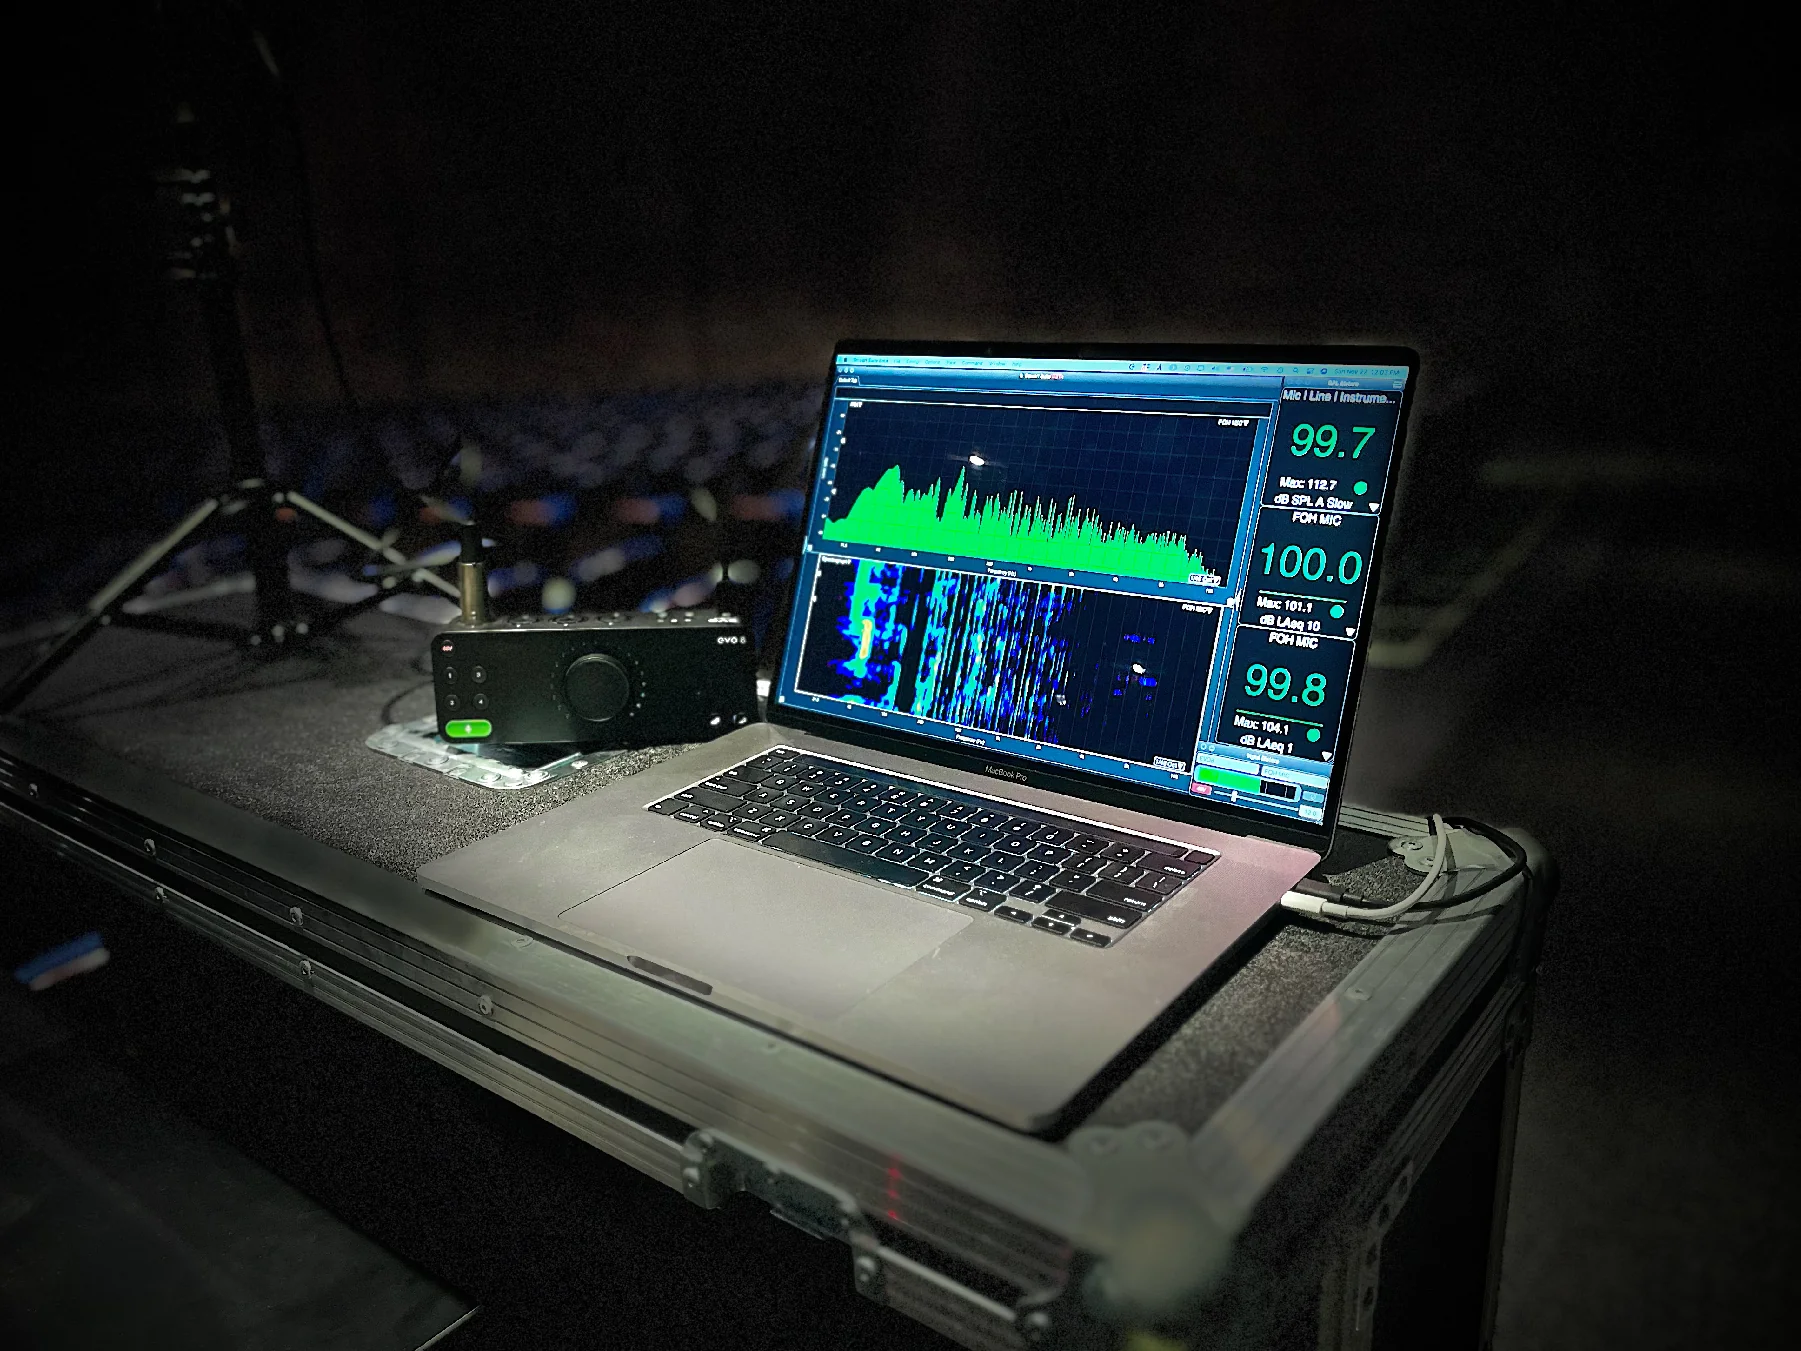
\includegraphics[width=0.9
	\linewidth]{Figures/smaart_01.png}
	\caption{Notebook using Smaart, where we can see some of the tools it includes. The notebook is connected to the EVO 8 (a USB interface that acts as an external sound card).}
	\label{fig:SMAART}
\end{figure}
	
The strongest points of this program are:

\begin{itemize}
	\item \textbf{Flexibility:} As a software-based solution, it can run on any Windows or Mac computer (meeting the minimum required specs), and can be used with most external audio sound cards, allowing the connection of unlimited types of microphones or direct signals.
	
	\item \textbf{More than one channel:} This software can analyze and display information from more than one input channel at the same time, allowing comparisons between different channels. This is used to compare an original signal with the signal captured by a microphone inside a room with a sound system, helping to detect room acoustics or sound system issues. Another common use is to measure the sound in different places of the same room simultaneously.
	
	\item \textbf{Widely used:} It is very common to see professionals in the sector using this software, or at least being familiar with it. It has become a kind of standard, which leads other companies to ensure maximum compatibility with it. For example, Audix makes the Audix TM-1 Plus microphone \cite{AudixTM1}, which includes a file that can be imported into SMAART to apply microphone correction during analysis.
\end{itemize}


On the other hand, it requires a license, external hardware such as sound cards and microphones, and it does not have any correction capabilities—only analysis.


\section{Dirac Live}

\textbf{Dirac Live} \cite{dirac_live} is a software-based solution focused on room correction in home environments, aimed at users who want to improve the sound quality of their home theater systems or other audio setups without applying structural acoustic treatments. In many cases, it's not possible to perform physical acoustic modifications at home, so this software helps address such limitations by digitally correcting the room’s response or enhancing the speaker performance.

Since it includes a correction processor, Dirac requires a dedicated computer to run continuously and process the audio being played through the system. Users can either use their own PC for this purpose or purchase a dedicated hardware unit provided by the company.

Additionally, setting up this solution requires a measurement microphone connected to the system, which captures the room and speaker response using excitation signals generated by the program itself. Dirac recommends specific microphones for this task and allows the import of calibration files to correct for minor microphone imperfections. Even so, it is acceptable to use other microphones as long as they come with measurement specifications, allowing for reasonably accurate results.

\begin{figure}[H]
	\centering
	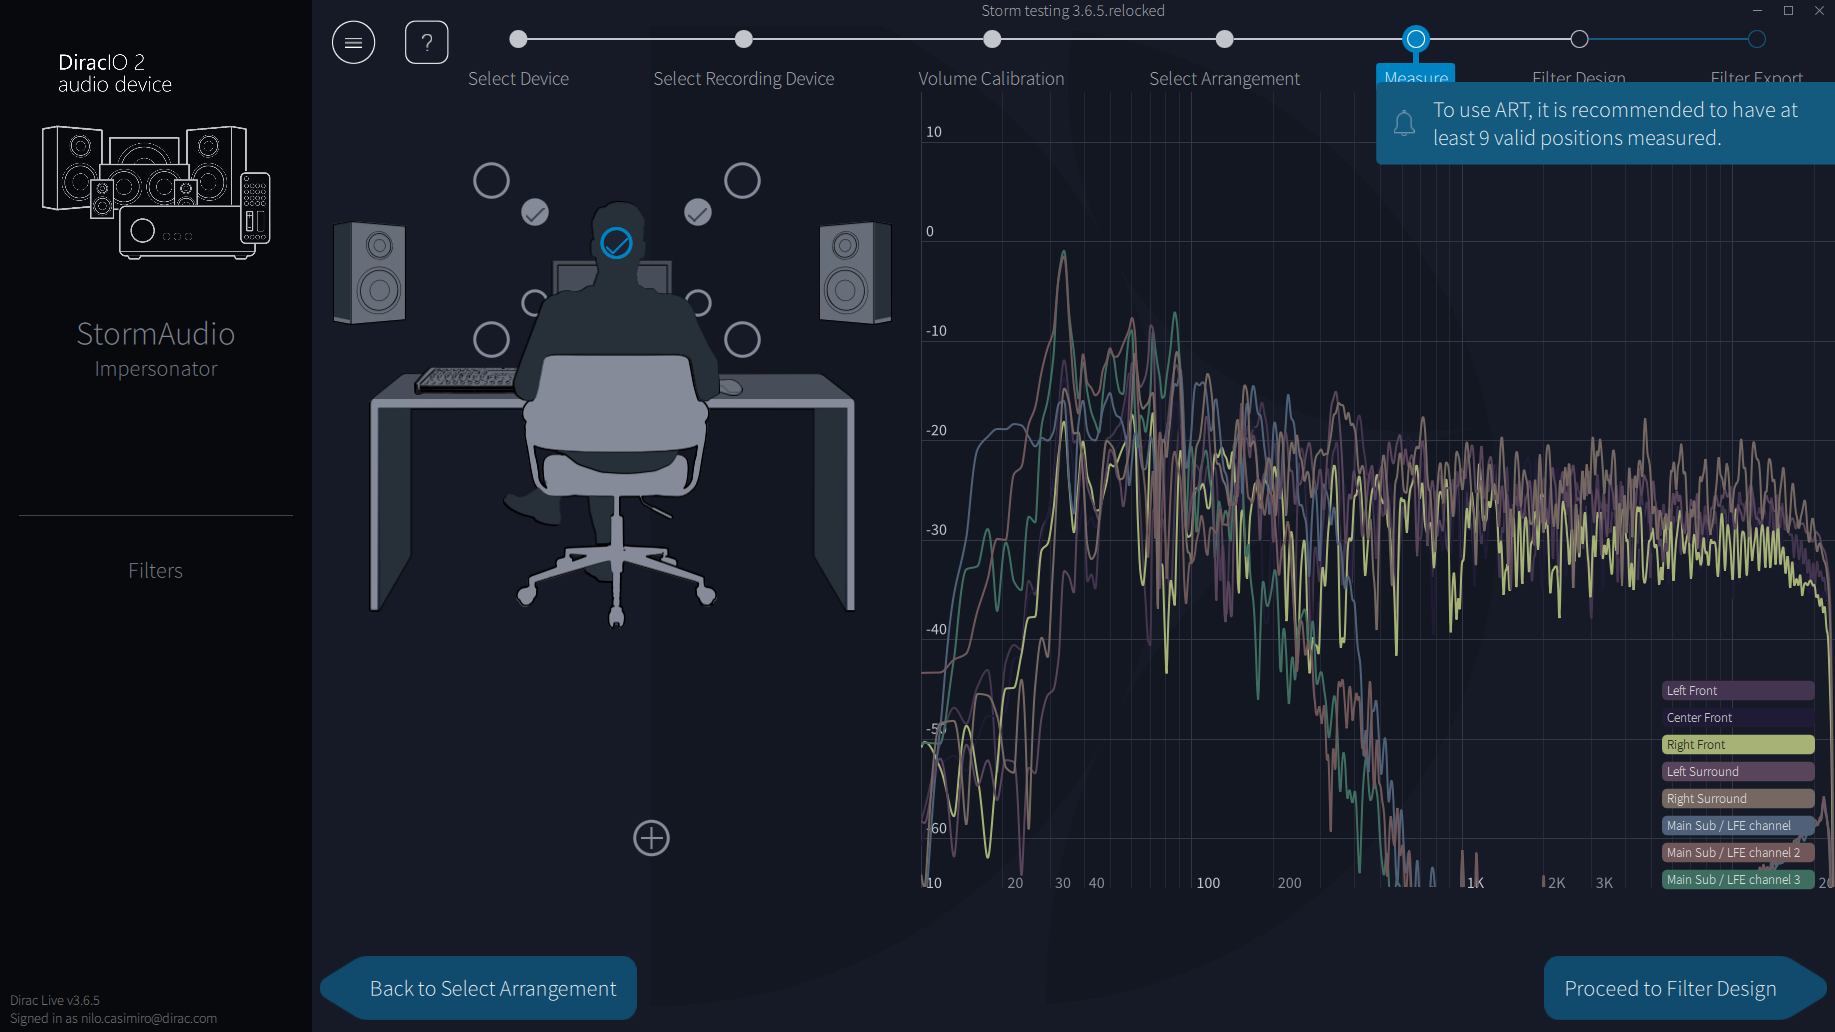
\includegraphics[width=0.9
	\linewidth]{Figures/dirac.jpg}
	\caption{Screenshot of Dirac Live software.}
	\label{fig:Dirac}
\end{figure}

As with any other solution, it has its downsides and upsides:

\begin{itemize}
	\item On one hand, the biggest downside of this solution, in my opinion, is that it is heavily focused on users with little or no technical knowledge. While this is great because it makes the software easy to use and more accessible to any enthusiast, it also makes the system very opaque. You cannot know exactly what kind of correction is being applied or what analysis results the correction is based on. It provides very little information about what it is actually doing.
	
	\item On the other hand, the biggest upside is its broad compatibility with many different multichannel system configurations, such as Stereo, LCR, Mono, 5.1, 6.0, 7.1, 5.1.2, and many more. Additionally, it can run as a standalone program, as a plugin within a DAW (\textit{Digital Audio Workstation}), or even on dedicated hardware. Finally, it is very easy to use. All of these features make it a highly flexible and appealing solution.
\end{itemize}

To use Dirac Live, it is necessary to purchase a license. The company offers different license tiers that enable or restrict certain features, allowing the price to be adapted to different use cases and user needs.


\section{Trinnov}

\textbf{Trinnov}\cite{trinnov} is an expensive hardware-based solution with a complex correction module, aimed at high-end professional studios and premium home theaters. Unlike software-only solutions such as Dirac Live, Trinnov provides dedicated processing units that integrate directly into the audio signal chain. These units handle tasks such as room correction, speaker alignment, and advanced phase and delay compensation in real time.

\begin{figure}[H]
	\centering
	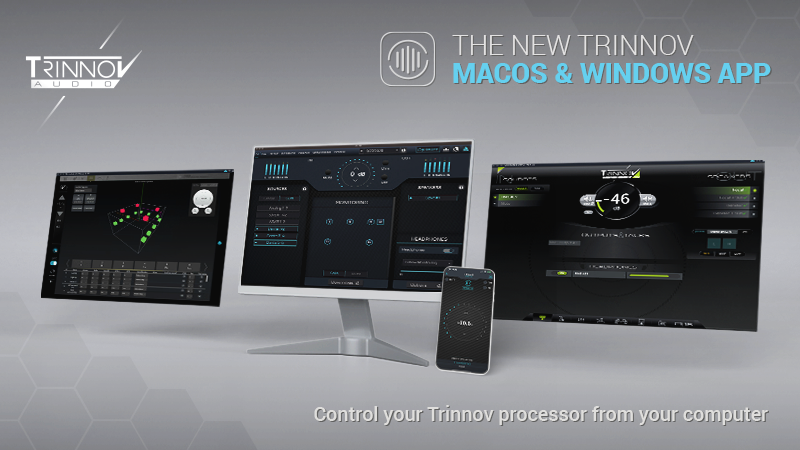
\includegraphics[width=0.9
	\linewidth]{Figures/trinnov_soft.png}
	\caption{Software used to configure and control Trinnov hardware processors.}
	\label{fig:trinnov_soft}
\end{figure}

An important particularity of this system is that it requires a specific and complex microphone provided by the same manufacturer. This microphone includes four measurement capsules arranged in a precise spatial configuration, allowing the system to determine the direction of incoming sound in a 3D space. This spatial information is used to correct complex acoustic issues and to create virtual sound sources, enhancing the immersive characteristics of the sound system within a specific room.

\begin{figure}[H]
	\centering
	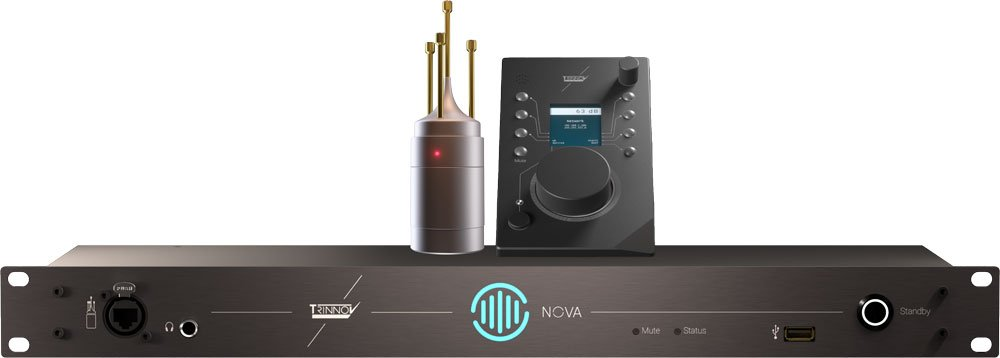
\includegraphics[width=0.9
	\linewidth]{Figures/trinnov_set.jpg}
	\caption{Commercial set including a hardware processor, a proprietary four-capsule microphone, and a desktop remote control.}
	\label{fig:trinnov_hard}
\end{figure}

It is also highly flexible, offering a wide range of options and detailed control. This solution is considered one of the most precise and reliable systems for digitally improving the acoustics of a room.

On the downside, Trinnov is significantly more expensive than most alternatives, as it relies on dedicated hardware and proprietary measurement tools. This cost places it outside the range of many semi-professional or enthusiast users.


\section{Other Solutions}

There are many more solutions available, but most of them are similar or offer the same tools with a similar workflow. However, I consider the following ones particularly worth mentioning:

\begin{itemize}
	\item \textbf{REW} (Room EQ Wizard)\cite{rew} is a free software-based solution that competes directly with \textbf{SMAART}, offering very similar features. However, it is more focused on non-live situations, such as studio or home audio analysis.

	\item \textbf{SoundID Reference} from the company Sonarworks \cite{soundID} is a software-based solution similar to \textbf{Dirac Live}, but more focused on home studio environments. It includes more advanced configuration options and offers additional features, such as a headphone calibration tool.
	
\end{itemize}


